\section{Previous meetings}

\subsection{Network structure}

\cref{tab:results-previous-meetings-accuracy} shows the \gls{rps} values and accuracy of the previous meetings network. In the evaluation data set, 38.1\% of all matches ended in a home victory.
\begin{table}
    \centering
    \begin{tabulary}{\textwidth}{| L | L || L | L | L || L |}
        \hline
        \multicolumn{2}{| l ||}{\textbf{Hidden layer}}  & \multicolumn{3}{l ||}{\textbf{\gls{rps} values}} & \\\hline
        \textbf{Activation} & \textbf{Size}             & \textbf{Min}  & \textbf{Max}  & \textbf{Mean} & \textbf{Accuracy} \\\hline
        \gls{relu}          & 32                        & 0.0525        & 0.585         & 0.235         & 0.374 \\\hline
        \gls{relu}          & 64                        & 0.0425        & 0.616         & 0.236         & 0.381 \\\hline
        \gls{relu}          & 128                       & 0.0505        & 0.616         & 0.242         & 0.358 \\\hline
        
        \hline
        
        Sigmoid             & 32                        & 0.125         & 0.457         & 0.228         & 0.374 \\\hline
        Sigmoid             & 64                        & 0.138         & 0.436         & 0.236         & 0.381 \\\hline
        Sigmoid             & 128                       & 0.133         & 0.371         & 0.228         & 0.381 \\\hline
        Sigmoid             & 256                       & 0.112         & 0.484         & 0.230         & 0.381 \\\hline
        
        \hline
        
        \Gls{tanh}          & 32                        & 0.0342        & 0.650         & 0.249         & 0.354 \\\hline
        \Gls{tanh}          & 64                        & 0.0573        & 0.619         & 0.237         & 0.361 \\\hline
        \rowcolor{correct}
        \Gls{tanh}          & 128                       & 0.0352        & 0.646         & 0.236         & 0.394 \\\hline
        \Gls{tanh}          & 256                       & 0.0340        & 0.671         & 0.248         & 0.381 \\\hline
    \end{tabulary}
    \caption{Accuracy of the previous meetings network, with different hidden layer configurations. The row colored green shows the configuration with most promising results.}
    \label{tab:results-previous-meetings-accuracy} 
\end{table}

Using a hidden layer with 128 nodes activated by the \gls{tanh} function yielded the most promising results, and will therefore be used when evaluating the profitability of the network. \cref{tab:results-previous-meetings-accuracy-2016-2017} shows the \gls{rps} values and prediction accuracy when evaluating the same configuration over the 2016-2017 season. Unfortunately, the network did not perform better than the benchmark model for any of the seasons.
\begin{table}
    \centering
    \begin{tabulary}{\textwidth}{| L | L | L || L |}
        \hline
        \multicolumn{3}{| l ||}{\textbf{\gls{rps} values}}  &                   \\\hline
        \textbf{Min}    & \textbf{Max}  & \textbf{Mean}     & \textbf{Accuracy} \\\hline
        0.0807          & 0.657         & 0.217             & 0.503             \\\hline
    \end{tabulary}
    \caption{Prediction accuracy of the previous meetings network for the 2016-2017 season of the English Premier League, using the most promising hidden layer configuration.}
    \label{tab:results-previous-meetings-accuracy-2016-2017} 
\end{table}


\subsection{Betting results}

\subsubsection{English Premier League 2015-2016}

\cref{fig:results-previous-meetings-2015-2016-fixed-bet,fig:results-previous-meetings-2015-2016-fixed-return,fig:results-previous-meetings-2015-2016-kelly-ratio,fig:results-previous-meetings-2015-2016-variance-adjusted} show the development of the \gls{roi} generated by the previous meetings network over the English Premier League season 2015-2016.
\begin{figure}
    \centering
    \includegraphics[width=\textwidth]{results/previous-meetings/2015-2016/fixed-bet-10.png}
    \caption{\gls{roi} over the span of the English Premier League season 2015-2016 using the previous meetings network and the fixed bet strategy.}
    \label{fig:results-previous-meetings-2015-2016-fixed-bet}
\end{figure}
\begin{figure}
    \centering
    \includegraphics[width=\textwidth]{results/previous-meetings/2015-2016/fixed-return-10.png}
    \caption{\gls{roi} over the span of the English Premier League season 2015-2016 using the previous meetings network and the fixed return strategy.}
    \label{fig:results-previous-meetings-2015-2016-fixed-return}
\end{figure}
\begin{figure}
    \centering
    \includegraphics[width=\textwidth]{results/previous-meetings/2015-2016/kelly-ratio-10.png}
    \caption{\gls{roi} over the span of the English Premier League season 2015-2016 using the previous meetings network and the Kelly ratio strategy.}
    \label{fig:results-previous-meetings-2015-2016-kelly-ratio}
\end{figure}
\begin{figure}
    \centering
    \includegraphics[width=\textwidth]{results/previous-meetings/2015-2016/variance-adjusted-10.png}
    \caption{\gls{roi} over the span of the English Premier League season 2015-2016 using the previous meetings network and the variance adjusted strategy.}
    \label{fig:results-previous-meetings-2015-2016-variance-adjusted}
\end{figure}

\cref{tab:fig:results-previous-meetings-2015-2016-roi} shows a summary of the \gls{roi} values achieved by the different strategies when used by the previous meetings network. The table shows the final \gls{roi} for the least profitable and most profitable simulations, together with the average final \gls{roi}.
\begin{table}
    \centering
    \begin{tabulary}{\textwidth}{| L || L | L | L |}
        \hline
                            & \multicolumn{3}{l |}{\textbf{Final \gls{roi}}} \\\hline
        \textbf{Strategy}   & \textbf{Min}  & \textbf{Max}  & \textbf{Mean} \\\hline
        Fixed bet           & -0.17         & 0.62          & 0.25 \\\hline
        Fixed return        & -0.13         & 0.099         & -0.012 \\\hline
        Kelly ratio         & -1.0          & 3.1           & \cellcolor{correct} 1.2 \\\hline
        Variance adjusted   & -0.17         & 0.075         & -0.052 \\\hline
    \end{tabulary}
    \caption{Final \gls{roi} values for the four strategies when using the previous meetings network during the 2015-2016 season of the English Premier League. The green colored cell was the most profitable strategy (on average).}
    \label{tab:fig:results-previous-meetings-2015-2016-roi}
\end{table}
     
\cref{fig:results-previous-meetings-2015-2016-odds-prob} shows the bets placed during the 2015-2016 season of the English Premier League. The probabilities are generated by a random instance of the previous meetings network.
\begin{figure}
    \centering
    \includegraphics[width=\textwidth]{results/previous-meetings/2015-2016/odds-prob.png}
    \caption{Offered odds and predicted probabilities for the bets placed during the 2015-2016 season of the English Premier League. The probabilities are generated by the previous meetings network.}
    \label{fig:results-previous-meetings-2015-2016-odds-prob}
\end{figure}
   

\subsubsection{English Premier League 2016-2017}

\cref{fig:results-previous-meetings-2016-2017-fixed-bet,fig:results-previous-meetings-2016-2017-fixed-return,fig:results-previous-meetings-2016-2017-kelly-ratio,fig:results-previous-meetings-2016-2017-variance-adjusted} show the development of the \gls{roi} generated by the previous meetings network over the English Premier League season 2016-2017.
\begin{figure}
    \centering
    \includegraphics[width=\textwidth]{results/previous-meetings/2016-2017/fixed-bet-10.png}
    \caption{\gls{roi} over the span of the English Premier League season 2016-2017 using the previous meetings network and the fixed bet strategy.}
    \label{fig:results-previous-meetings-2016-2017-fixed-bet}
\end{figure}
\begin{figure}
    \centering
    \includegraphics[width=\textwidth]{results/previous-meetings/2016-2017/fixed-return-10.png}
    \caption{\gls{roi} over the span of the English Premier League season 2016-2017 using the previous meetings network and the fixed return strategy.}
    \label{fig:results-previous-meetings-2016-2017-fixed-return}
\end{figure}
\begin{figure}
    \centering
    \includegraphics[width=\textwidth]{results/previous-meetings/2016-2017/kelly-ratio-10.png}
    \caption{\gls{roi} over the span of the English Premier League season 2016-2017 using the previous meetings network and the Kelly ratio strategy.}
    \label{fig:results-previous-meetings-2016-2017-kelly-ratio}
\end{figure}
\begin{figure}
    \centering
    \includegraphics[width=\textwidth]{results/previous-meetings/2016-2017/variance-adjusted-10.png}
    \caption{\gls{roi} over the span of the English Premier League season 2016-2017 using the previous meetings network and the variance adjusted strategy.}
    \label{fig:results-previous-meetings-2016-2017-variance-adjusted}
\end{figure}

\cref{tab:fig:results-previous-meetings-2016-2017-roi} shows a summary of the \gls{roi} values achieved by the different strategies when used by the previous meetings network. The table shows the final \gls{roi} for the least profitable and most profitable simulations, together with the average final \gls{roi}.
\begin{table}
    \centering
    \begin{tabulary}{\textwidth}{| L || L | L | L |}
        \hline
                            & \multicolumn{3}{l |}{\textbf{Final \gls{roi}}} \\\hline
        \textbf{Strategy}   & \textbf{Min}  & \textbf{Max}  & \textbf{Mean} \\\hline
        Fixed bet           & -0.48         & -0.15         & -0.34 \\\hline
        Fixed return        & -0.09         & 0.0055        & -0.050 \\\hline
        Kelly ratio         & -1.0          & -1.0          & -1.0 \\\hline
        Variance adjusted   & -0.058        & 0.027         & \cellcolor{correct} -0.022 \\\hline
    \end{tabulary}
    \caption{Final \gls{roi} values for the four strategies when using the previous meetings network during the 2016-2017 season of the English Premier League. The green colored cell was the most profitable strategy (on average).}
    \label{tab:fig:results-previous-meetings-2016-2017-roi}
\end{table}

\cref{fig:results-previous-meetings-2016-2017-odds-prob} shows the bets placed during the 2016-2017 season of the English Premier League. The probabilities are generated by a random instance of the previous meetings network.
\begin{figure}
    \centering
    \includegraphics[width=\textwidth]{results/previous-meetings/2016-2017/odds-prob.png}
    \caption{Offered odds and predicted probabilities for the bets placed during the 2016-2017 season of the English Premier League. The probabilities are generated by the previous meetings network.}
    \label{fig:results-previous-meetings-2016-2017-odds-prob}
\end{figure}


\subsubsection{Summary}

Similarly to the head to head network, the previous meetings network did not achieve consistent good results. The first season, the fixed bet and Kelly ratio strategies performed well, gaining a profit on average. The second season, however, the same strategies achieved \glspl{roi} of -0.34 and -1.0, respectively.

\cref{fig:results-previous-meetings-2015-2016-odds-prob,fig:results-previous-meetings-2016-2017-odds-prob} show the connection between odds and probabilities predicted by the previous meetings network. The previous meetings network has a more even spread than the head to head network. However, the previous meetings network tend to overestimate the probabilities across the board. The reason for the low spread is probably the same as for the head to head network. However, the previous meetings network also utilizes team ratings, accounting for potential team changes between the seasons. Over the two seasons, the prediction models won approximately 20.3\% of all bets placed, with an average odds of 4.70.